\section{Introduction}

% What is the problem?
File system metadata services in HPC have scalability problems because
administrative tasks, like checkpointing~\cite{bent_plfs_2009} or scanning the
file system~\cite{zheng:pdsw2014-batchfs}, contend for the same directories and
inodes. Applications perform better with dedicated metadata
servers~\cite{sevilla:sc15-mantle, ren:sc2014-indexfs} but provisioning a
metadata server for every client is unreasonable. This problem is exacerbated
by current trends in HPC, where architectures are transitioning from complex
storage stacks with burst buffer, file system, object store, and tape tiers to
more simplified stacks with just a burst buffer and object
store~\cite{bent:login16-hpc-trends}; this puts more pressure on data access
because more requests end up hitting the same layer and latencies cannot be
hidden while data migrates across tiers.

\begin{figure}[tb]
\centering
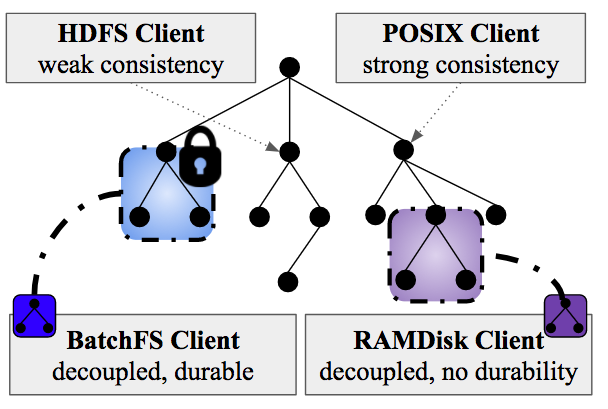
\includegraphics[width=0.35\textwidth]{figures/subtree-policies1.png}

\caption{For performance, clients can relax consistency on their subtree
({e.g.}, HDFS) or even decouple the subtree and move it locally ({e.g.},
BatchFS, RAMDisk). Decoupled subtrees can further relax durability semantics
for even better performance. Clients that require stronger guarantees ({\it
e.g.,} POSIX) can still reside in the same namespace.
}\label{fig:subtree-policies}

\end{figure}

% What is HPC doing?
To address this, developers are relaxing the consistency and durability
semantics in the file system because weaker guarantees are sufficient for their
applications. For example, many batch style jobs do not need the strong
consistency that the file system provides, so
BatchFS~\cite{zheng:pdsw2014-batchfs} and DeltaFS~\cite{zheng:pdsw2015-deltafs}
do more client-side processing and merge updates when the job is done. HPC
developers are turning to these non-POSIX solutions because their applications
are well-understood ({\it e.g.}, well-defined read/write phases,
synchronization only needed during certain phases, workflows describing
computation, etc.) and because these applications wreak havoc on file systems designed for
general-purpose workloads ({\it e.g.}, checkpoint-restart's N-N and N-1 create
patterns).

% One example
One popular approach for relaxing consistency and durability is to ``decouple
the namespace", where clients lock the subtree they want exclusive access to as
a way to tell the file system that the subtree is important or may cause
resource contention in the near-future~\cite{grider:pdsw2015-marfs,
zheng:pdsw2015-deltafs, zheng:pdsw2014-batchfs, ren:sc2014-indexfs,
bent:slides-twotiers}. Then the file system can change its internal structure
to optimize performance. For example, the file system could enter a mode that
prevents other clients from interfering with the decoupled directory.  This
delayed merge ({\it i.e.} a form of eventual consistency) and relaxed
durability improves performance and scalability by avoiding the costs of remote
procedure calls (RPCs), synchronization, false sharing, and serialization.
While the performance benefits of decoupling the namespace are obvious,
applications that rely on the file system's guarantees must be deployed on an
entirely different system or re-written to coordinate strong
consistency/durability themselves.

%\begin{table}
%\begin{tabular}{ r | l }
%  Subtree         & Example \\\hline
%  (1)   & \{Index, Batch\}FS~\cite{ren:sc2014-indexfs, zheng:pdsw2014-batchfs} \\
%  (2)   & \{Index, Ceph\}FS~\cite{ren:sc2014-indexfs, weil:sc2004-dyn-metadata} \\
%  (3)   & RAMDisk \\
%  (4)   & DeltaFS~\cite{zheng:pdsw2015-deltafs} \\
%\end{tabular}
%
%\caption{State-of-the-art systems in HPC improve file system metadata
%performance by relaxing consistency and durability guarantees. Note that
%IndexFS also supports weak consistency with bulk inserts.
%\label{table:namespaces}} \end{table}

% What did we do
To address this problem, we present an API and framework that lets developers
dynamically control the consistency and durability guarantees for subtrees in
the file system namespace.  Figure~\ref{fig:subtree-policies} shows a setup in
our proposed system where a single global namespace has subtrees for
applications optimized with techniques from different state-of-the-art HPC
architectures.  The HDFS\footnote{This is example is not directly evaluated in
this paper, although a similar use case is explored in~\S\ref{use-case-1}}
subtree has weaker consistency than strong consistency because it  does not
guarantee that all updates are not immediately seen by all servers; the BatchFS
and RAMDisk subtrees are decoupled from the global namespace and have similar
consistency/durability behavior to those systems; and the POSIX subtree retains
the rigidity of POSIX's strong consistency.

Our prototype system, Cudele, achieves this by exposing ``mechanisms" that
developers use to specify their preferred semantics.  Cudele supports 3 forms
of consistency (invisible, weak, and strong) and 3 degrees of durability (none,
local, and global) giving the user a wide range of policies and optimizations
that can be custom fit to an application. We make the following contributions:

\begin{enumerate}

  \item a prototype that lets developers choose from a range of
  consistency and durability semantics (9 permutations), allowing them to dynamically custom
  fit the storage system to the application.

  \item an API for selecting consistency/durability policies and assigning
  them to subtrees in the file system namespace.

  \item an apples-to-apples comparison of the strategies used in recently proposed research systems against
  previously unexplored metadata designs, all implemented using Cudele.

\end{enumerate}

% Results
Our results confirm the assertions of ``clean-state" research systems that
decouple namespaces; specifically that the technique drastically improves
performance (104\(\times\) speed up) but we go a step further by quantifying
the costs of merging updates (7\(\times\) slow down) and maintaining durability
(\(10\times\) slow down). We also show the effect of having a metadata specific
file format in systems that are based on in-memory data structures.  We scale
up to 20 clients executing an extremely metadata intensive job because this
workload exhausts the resources of a single metadata server for the code base we
built on.  Partitioning and replicating metadata across a cluster can be
controlled with something like Mantle~\cite{sevilla:sc15-mantle}, but in this
paper we show the capacity and performance of a metadata server with superior
metadata protocols, which should be used to inform load balancing decisions.

In the remainder of the paper, Section~\ref{sec:posix-overheads} quantifies the
cost of POSIX consistency and system-defined durability and
Section~\ref{sec:methodology-decoupled-namespaces} presents the Cudele
prototype and API. Section~\ref{sec:implementation} describes the Cudele
mechanisms and shows how re-using internal subsystems results in an
implementation of less than 500 lines of code. The evaluation in
Section~\ref{sec:evaluation} quantifies the overheads and performance gains of
explored and previously unexplored metadata designs.
Section~\ref{sec:related-work} places Cudele in the context of other related
work.

